\documentclass[11pt,a4paper]{report}
\usepackage[textwidth=37em,vmargin=30mm]{geometry}
\usepackage{calc,xunicode,amsmath,amssymb,paralist,enumitem,tabu,booktabs,datetime2,xeCJK,xeCJKfntef,listings}
\usepackage{tocloft,fancyhdr,tcolorbox,xcolor,graphicx,eso-pic,xltxtra,xelatexemoji}

\newcommand{\envyear}[0]{2025}
\newcommand{\envdatestr}[0]{2025-08-13}
\newcommand{\envfinaldir}[0]{webdb/2025/20250813/final}

\usepackage[hidelinks]{hyperref}
\hypersetup{
    colorlinks=false,
    pdfpagemode=FullScreen,
    pdftitle={Web Digest - \envdatestr}
}

\setlength{\cftbeforechapskip}{10pt}
\renewcommand{\cftchapfont}{\rmfamily\bfseries\large\raggedright}
\setlength{\cftbeforesecskip}{2pt}
\renewcommand{\cftsecfont}{\sffamily\small\raggedright}

\setdefaultleftmargin{2em}{2em}{1em}{1em}{1em}{1em}

\usepackage{xeCJK,xeCJKfntef}
\xeCJKsetup{PunctStyle=plain,RubberPunctSkip=false,CJKglue=\strut\hskip 0pt plus 0.1em minus 0.05em,CJKecglue=\strut\hskip 0.22em plus 0.2em}
\XeTeXlinebreaklocale "zh"
\XeTeXlinebreakskip = 0pt


\setmainfont{Brygada 1918}
\setromanfont{Brygada 1918}
\setsansfont{IBM Plex Sans}
\setmonofont{JetBrains Mono NL}
\setCJKmainfont{Noto Serif CJK SC}
\setCJKromanfont{Noto Serif CJK SC}
\setCJKsansfont{Noto Sans CJK SC}
\setCJKmonofont{Noto Sans CJK SC}

\setlength{\parindent}{0pt}
\setlength{\parskip}{8pt}
\linespread{1.15}

\lstset{
	basicstyle=\ttfamily\footnotesize,
	numbersep=5pt,
	backgroundcolor=\color{black!5},
	showspaces=false,
	showstringspaces=false,
	showtabs=false,
	tabsize=2,
	captionpos=b,
	breaklines=true,
	breakatwhitespace=true,
	breakautoindent=true,
	linewidth=\textwidth
}






\newcommand{\coverpic}[2]{
    % argv: itemurl, authorname
    Cover photo by #2~~(\href{#1}{#1})
}
\newcommand{\makeheader}[0]{
    \begin{titlepage}
        % \newgeometry{hmargin=15mm,tmargin=21mm,bmargin=12mm}
        \begin{center}
            
            \rmfamily\scshape
            \fontspec{BaskervilleF}
            \fontspec{Old Standard}
            \fontsize{59pt}{70pt}\selectfont
            WEB\hfill DIGEST
            
            \vfill
            % \vskip 30pt
            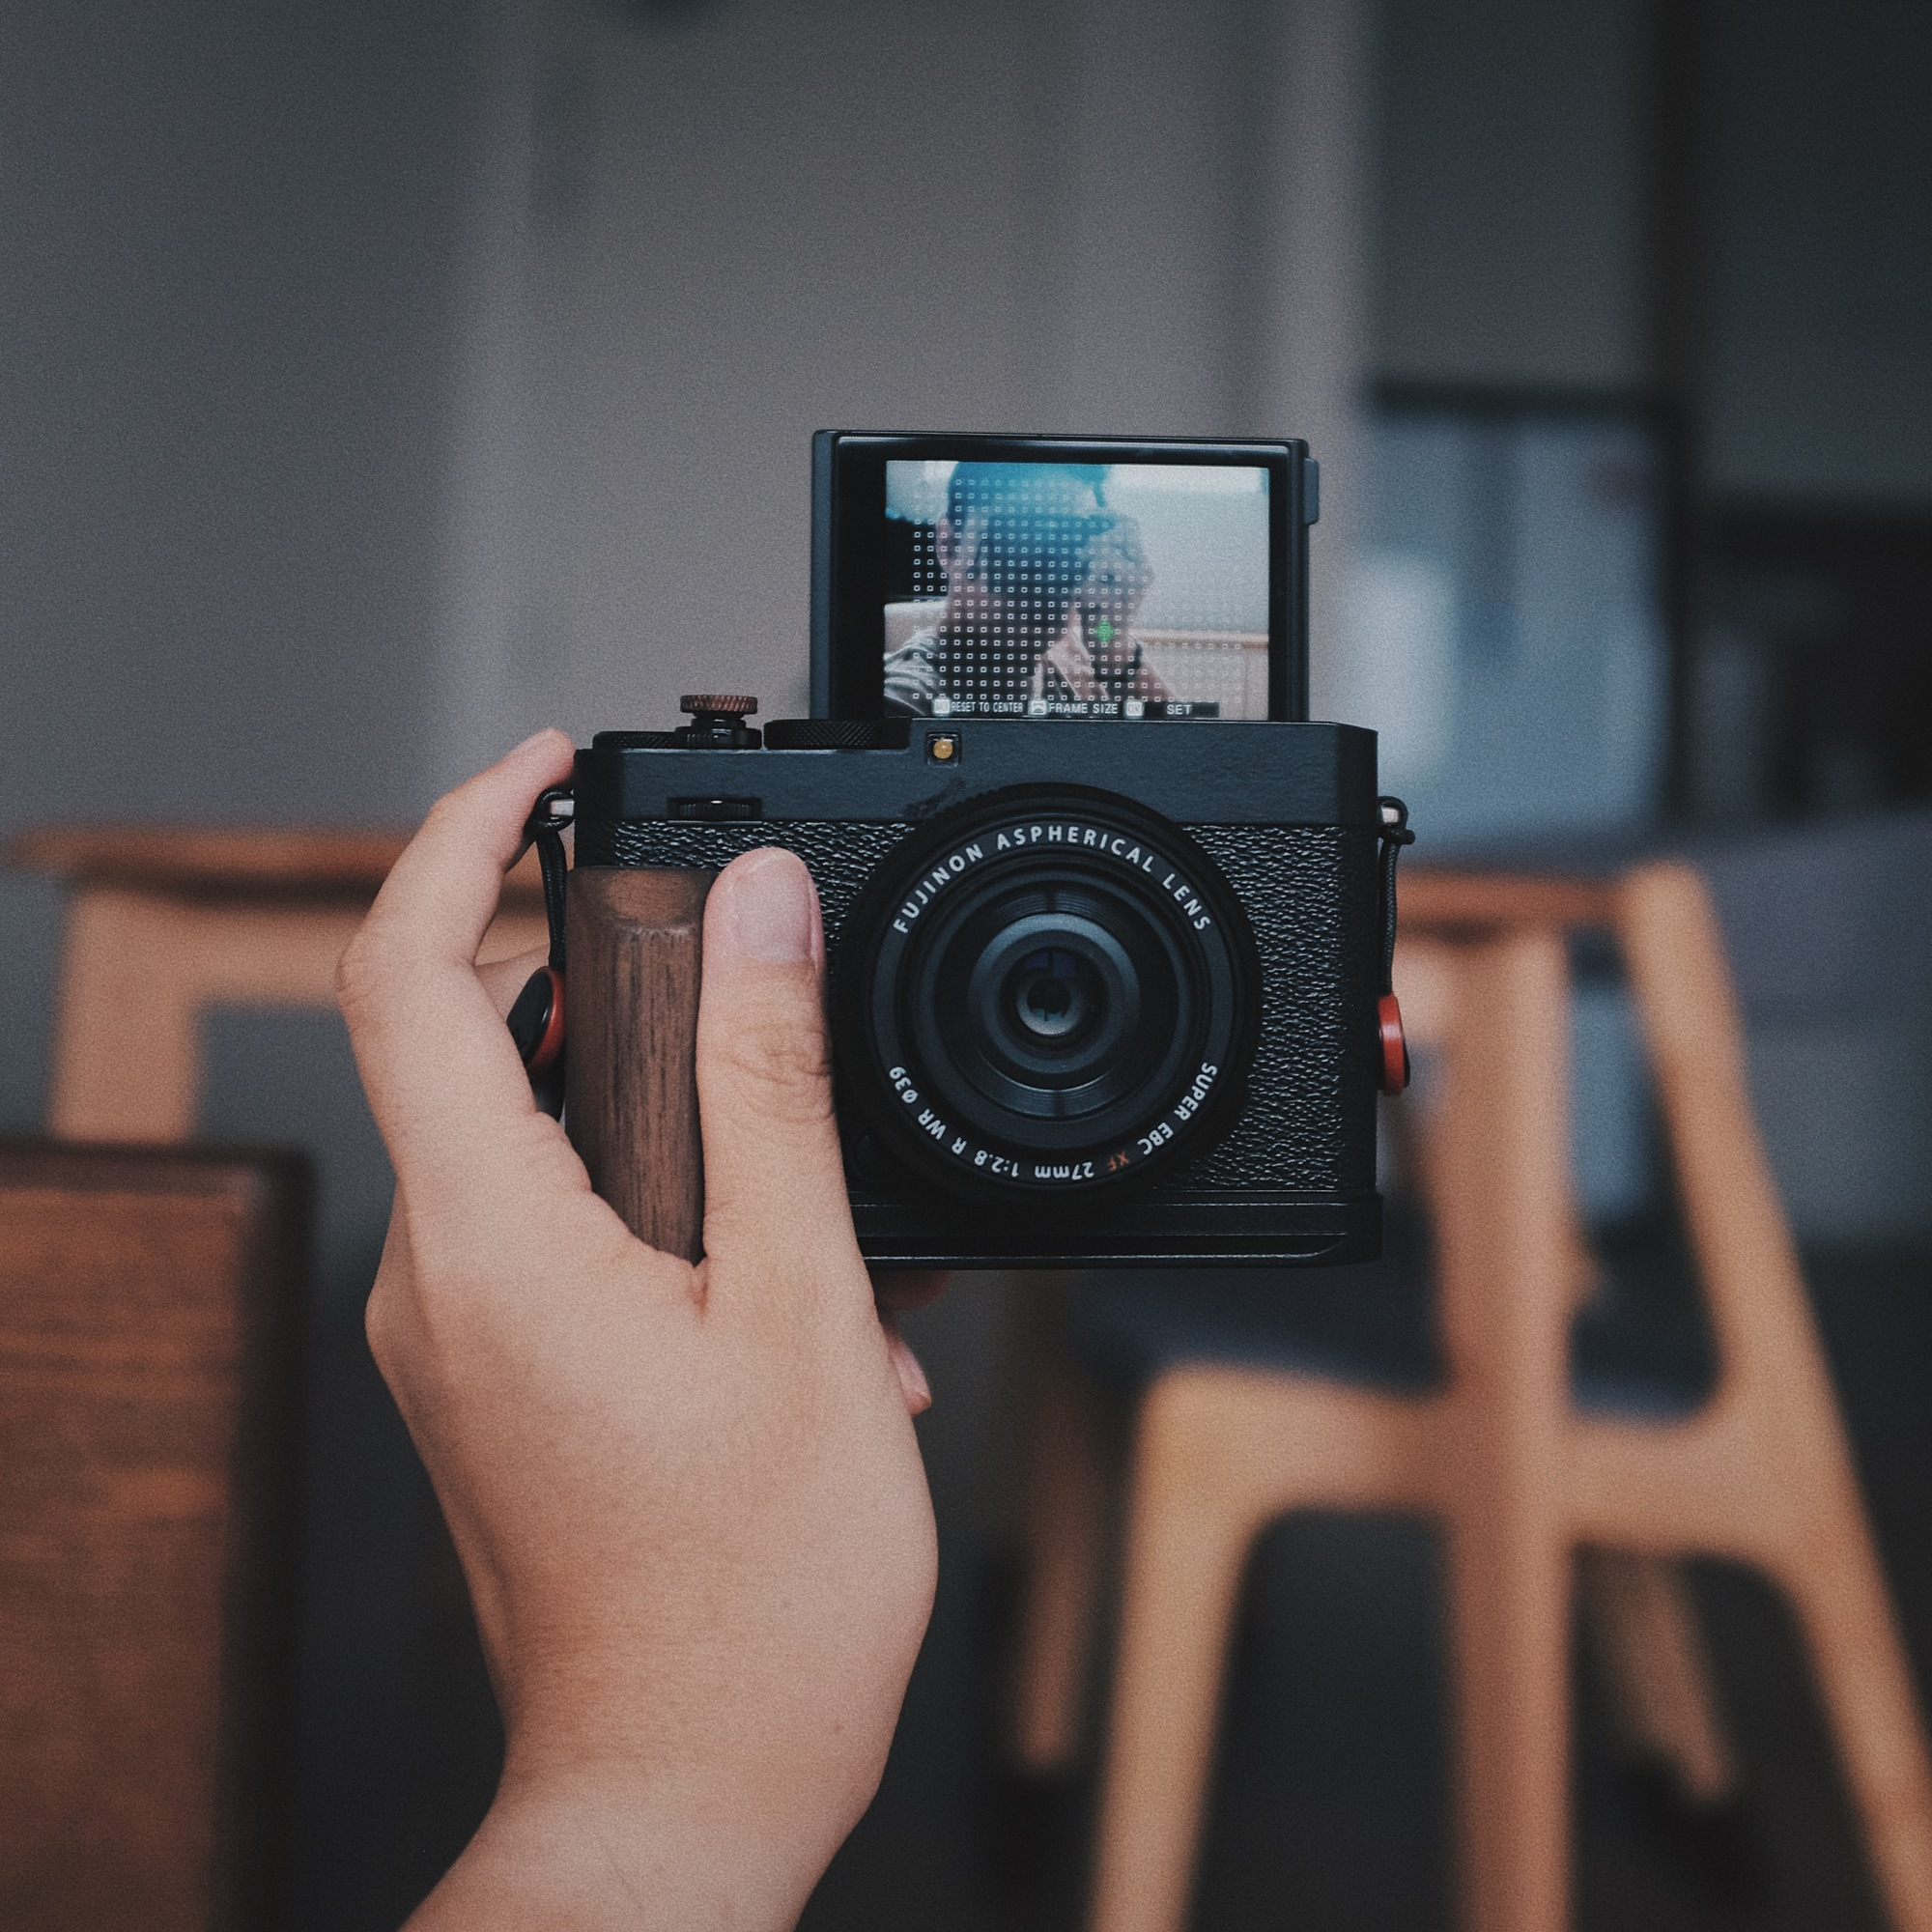
\includegraphics[width=\linewidth]{\envfinaldir/coverpic-prod.jpg}\par
            % \vskip 30pt
            \vfill

            \normalsize\rmfamily\scshape
            \copyright{} The Web Digest Project \hfill\large \envdatestr
        \end{center}
    \end{titlepage}
    % \restoregeometry
}
\newcommand{\simplehref}[1]{%
    \textcolor{blue!80!green}{\href{#1}{#1}}%
}
\renewcommand{\contentsname}{\center\Huge\sffamily\bfseries Contents\par\vskip 20pt}
\newcounter{ipartcounter}
\setcounter{ipartcounter}{0}
\newcommand{\ipart}[1]{
    % \vskip 20pt
    \clearpage
    \stepcounter{ipartcounter}
    \phantomsection
    \addcontentsline{toc}{chapter}{#1}
    % \begin{center}
    %     \Huge
    %     \sffamily\bfseries
    %     #1
    % \end{center}
    % \vskip 20pt plus 7pt
}
\newcounter{ichaptercounter}
\setcounter{ichaptercounter}{0}
\newcommand{\ichapter}[1]{
    % \vskip 20pt
    \clearpage
    \stepcounter{ichaptercounter}
    \phantomsection
    \addcontentsline{toc}{section}{\numberline{\arabic{ichaptercounter}}#1}
    \begin{center}
        \Huge
        \sffamily\bfseries
        #1
    \end{center}
    \vskip 20pt plus 7pt
}
\newcommand{\entrytitlefont}[1]{\subsection*{\raggedright\Large\sffamily\bfseries#1}}
\newcommand{\entryitemGeneric}[2]{
    % argv: title, url
    \parbox{\linewidth}{
        \entrytitlefont{#1}\par\vskip 5pt
        \footnotesize\ttfamily\mdseries
        \simplehref{#2}
    }\vskip 11pt plus 11pt minus 1pt
}
\newcommand{\entryitemGithub}[3]{
    % argv: title, url, desc
    \parbox{\linewidth}{
        \entrytitlefont{#1}\par\vskip 5pt
        \footnotesize\ttfamily\mdseries
        \simplehref{#2}\par\vskip 5pt
        \small\rmfamily\mdseries#3
    }\vskip 11pt plus 11pt minus 1pt
}
\newcommand{\entryitemAp}[3]{
    % argv: title, url, desc
    \parbox{\linewidth}{
        \entrytitlefont{#1}\par\vskip 5pt
        \footnotesize\ttfamily\mdseries
        \simplehref{#2}\par\vskip 5pt
        \small\rmfamily\mdseries#3
    }\vskip 11pt plus 11pt minus 1pt
}
\newcommand{\entryitemHackernews}[3]{
    % argv: title, hnurl, rawurl
    % \parbox{\linewidth}{
    %     \entrytitlefont{#1}\par\vskip 5pt
    %     \footnotesize\ttfamily\mdseries
    %     \simplehref{#3}\par
    %     \textcolor{black!50}{\href{#2}{#2}}
    % }\vskip 11pt plus 11pt minus 1pt
    \begin{minipage}{\linewidth}
            \entrytitlefont{#1}\par\vskip 5pt
            \footnotesize\ttfamily\mdseries
            \simplehref{#3}\par
            \textcolor{black!50}{\href{#2}{#2}}
    \end{minipage}\par\vskip 11pt plus 11pt minus 1pt
}







\begin{document}

\makeheader

\tableofcontents\clearpage




\ipart{Developers}
\ichapter{Hacker News}
\entryitemTwoLinks{Ashet Home Computer}{https://news.ycombinator.com/item?id=44880401}{https://ashet.computer/}

\entryitemTwoLinks{Let's get real about the one-person billion dollar company}{https://news.ycombinator.com/item?id=44879853}{https://www.marcrand.com/p/lets-get-real-about-the-one-person}

\entryitemTwoLinks{H-1B Visa Changes Approved by White House}{https://news.ycombinator.com/item?id=44879746}{https://www.newsweek.com/h-1b-visas-changes-approved-white-house-report-2112216}

\entryitemTwoLinks{Is the A.I. Boom Turning Into an A.I. Bubble?}{https://news.ycombinator.com/item?id=44879373}{https://www.newyorker.com/news/the-financial-page/is-the-ai-boom-turning-into-an-ai-bubble}

\entryitemTwoLinks{Claude vs. Gemini: Testing on 1M Tokens of Context}{https://news.ycombinator.com/item?id=44878999}{https://every.to/vibe-check/vibe-check-claude-sonnet-4-now-has-a-1-million-token-context-window}

\entryitemTwoLinks{Show HN: Omnara – Run Claude Code from anywhere}{https://news.ycombinator.com/item?id=44878650}{https://github.com/omnara-ai/omnara}

\entryitemTwoLinks{Show HN: Building a web search engine from scratch with 3B neural embeddings}{https://news.ycombinator.com/item?id=44878151}{https://blog.wilsonl.in/search-engine/}

\entryitemTwoLinks{Claude Sonnet 4 now supports 1M tokens of context}{https://news.ycombinator.com/item?id=44878147}{https://www.anthropic.com/news/1m-context}

\entryitemTwoLinks{Perplexity Makes Longshot \$34.5B Offer for Chrome}{https://news.ycombinator.com/item?id=44877656}{https://www.wsj.com/tech/perplexity-makes-longshot-34-5-billion-offer-for-chrome-5ddb7a22}

\entryitemTwoLinks{UK government advises deleting emails to save water}{https://news.ycombinator.com/item?id=44877292}{https://www.gov.uk/government/news/national-drought-group-meets-to-address-nationally-significant-water-shortfall}

\entryitemTwoLinks{The ex-CIA agents deciding Facebook's content policy (2022)}{https://news.ycombinator.com/item?id=44877221}{https://mronline.org/2022/07/14/meet-the-ex-cia-agents-deciding-facebooks-content-policy/}

\entryitemTwoLinks{Why are there so many rationalist cults?}{https://news.ycombinator.com/item?id=44877076}{https://asteriskmag.com/issues/11/why-are-there-so-many-rationalist-cults}

\entryitemTwoLinks{Enlisting in the Fight Against Link Rot}{https://news.ycombinator.com/item?id=44877021}{https://jszym.com/blog/archiving\_googl/}

\entryitemTwoLinks{GitHub was having issues}{https://news.ycombinator.com/item?id=44876784}{https://www.githubstatus.com/incidents/9rfydl2xdqqj}

\entryitemTwoLinks{That viral video of a 'deactivated' Tesla Cybertruck is a fake}{https://news.ycombinator.com/item?id=44876449}{https://www.theverge.com/tesla/757594/tesla-cybertruck-deactivated-viral-video-fake}

\entryitemTwoLinks{Training language models to be warm and empathetic makes them less reliable}{https://news.ycombinator.com/item?id=44875992}{https://arxiv.org/abs/2507.21919}

\entryitemTwoLinks{Australian court finds Apple, Google guilty of being anticompetitive}{https://news.ycombinator.com/item?id=44875961}{https://www.ghacks.net/2025/08/12/australian-court-finds-apple-google-guilty-of-being-anticompetitive/}

\entryitemTwoLinks{Monero appears to be in the midst of a successful 51\% attack}{https://news.ycombinator.com/item?id=44875109}{https://twitter.com/p3b7\_/status/1955173413992984988}

\entryitemTwoLinks{Radicle 1.3.0}{https://news.ycombinator.com/item?id=44874945}{https://radicle.xyz/2025/08/12/radicle-1.3.0}

\entryitemTwoLinks{Qodo CLI agent scores 71.2\% on SWE-bench Verified}{https://news.ycombinator.com/item?id=44874736}{https://www.qodo.ai/blog/qodo-command-swe-bench-verified/}\ichapter{Phoronix}
\entryitemGeneric{\hskip 0pt{}Linux Address Space Isolation "ASI" Revived After Lowering 70\% Performance Hit To 13\%}{https://www.phoronix.com/news/Linux-ASI-Lower-Overhead}

\entryitemGeneric{\hskip 0pt{}Intel CPU Microcode Updates Released For Six High Severity Vulnerabilities}{https://www.phoronix.com/news/Intel-CPU-Microcode-August-2025}

\entryitemGeneric{\hskip 0pt{}CodeWeavers CrossOver 25.1 Improves The Stability Of Microsoft Office On Linux}{https://www.phoronix.com/news/CrossOver-25.1-Released}

\entryitemGeneric{\hskip 0pt{}Linux Kernel Patched For AMD SEV-SNP Cache Coherency Vulnerability}{https://www.phoronix.com/news/SEV-SNP-Cache-Coherency-Issue}

\entryitemGeneric{\hskip 0pt{}AMD Ryzen AI Max+ 395 With Framework Desktop vs. Intel Core Ultra 9 285K Linux Performance}{https://www.phoronix.com/review/amd-ryzen-ai-max-arrow-lake}

\entryitemGeneric{\hskip 0pt{}Debian GNU/Hurd 2025 Released With Completed 64-bit Support, Rust Ported}{https://www.phoronix.com/news/Debian-GNU-Hurd-2025}

\entryitemGeneric{\hskip 0pt{}NVIDIA 580.76.05 Linux Driver Updates EGL Bits, Adds New MetaMode Attribute}{https://www.phoronix.com/news/NVIDIA-580.76.05-Linux}

\entryitemGeneric{\hskip 0pt{}ZLUDA Implements Kernel Cache Support To Help With Performance}{https://www.phoronix.com/news/ZLUDA-Kernel-Cache}

\entryitemGeneric{\hskip 0pt{}Itanium IA-64 Support May Revert Back To Being Deprecated/Obsolete For GCC 16}{https://www.phoronix.com/news/Itanium-IA-64-GCC-16-Obsolete}


\ipart{Developers~~~~(zh-Hans)}
\ichapter{Solidot}
\entryitemGeneric{\hskip 0pt{}沃茨对 YouTube 的欺诈诉讼停滞不前}{https://www.solidot.org/story?sid=82019}

\entryitemGeneric{\hskip 0pt{}CEO 辞职,GitHub 不再在微软内部独立运营}{https://www.solidot.org/story?sid=82018}

\entryitemGeneric{\hskip 0pt{}高危 WinRAR 0day 正被利用}{https://www.solidot.org/story?sid=82017}

\entryitemGeneric{\hskip 0pt{}年轻血清配合骨髓细胞逆转皮肤衰老}{https://www.solidot.org/story?sid=82016}

\entryitemGeneric{\hskip 0pt{}研究发现素食者癌症风险比肉食者低 12\%}{https://www.solidot.org/story?sid=82015}

\entryitemGeneric{\hskip 0pt{}量子流体首次观测到类似梵高名画《星空》的漩涡结构}{https://www.solidot.org/story?sid=82014}

\entryitemGeneric{\hskip 0pt{}Steam 创意工坊知名模组遭遇大规模恶意 DMCA 举报}{https://www.solidot.org/story?sid=82013}

\entryitemGeneric{\hskip 0pt{}Debian 14 考虑支持龙芯的 LoongArch CPU}{https://www.solidot.org/story?sid=82012}

\entryitemGeneric{\hskip 0pt{}Linux 6.17-rc1 释出,未合并 Bcachefs 任何补丁}{https://www.solidot.org/story?sid=82011}

\entryitemGeneric{\hskip 0pt{}中国制造了全球三分之一的常用塑料}{https://www.solidot.org/story?sid=82010}

\entryitemGeneric{\hskip 0pt{}澳大利亚大堡礁珊瑚白化创纪录}{https://www.solidot.org/story?sid=82009}

\entryitemGeneric{\hskip 0pt{}英伟达和 AMD 同意将 15\% 的中国营收上缴给美国}{https://www.solidot.org/story?sid=82008}

\entryitemGeneric{\hskip 0pt{}读卖新闻起诉 Perplexity 侵犯著作权}{https://www.solidot.org/story?sid=82006}

\entryitemGeneric{\hskip 0pt{}人与自然联结度 220 年来下降逾 60\%}{https://www.solidot.org/story?sid=82005}

\entryitemGeneric{\hskip 0pt{}安全加固的 Android 社区发行版 Graphene OS }{https://www.solidot.org/story?sid=82004}

\entryitemGeneric{\hskip 0pt{}Debian 13 trixie 释出}{https://www.solidot.org/story?sid=82003}

\entryitemGeneric{\hskip 0pt{}AI 淘汰初级编程开发者}{https://www.solidot.org/story?sid=82002}

\entryitemGeneric{\hskip 0pt{}签署捐赠誓言的 256 名亿万富翁只有 9 人信守诺言 }{https://www.solidot.org/story?sid=82001}\ichapter{V2EX}
\entryitemGeneric{\hskip 0pt{}[iOS] 有跟我一样 Safari 的``欺骗性网站警告''不知道什么时间自动打开的吗}{https://www.v2ex.com/t/1151966}

\entryitemGeneric{\hskip 0pt{}[Solana] \$V2EX 突然跌破 \$0.013 大家有赶上车吗?}{https://www.v2ex.com/t/1151965}

\entryitemGeneric{\hskip 0pt{}[分享创造] 明牌搞外链-分数计算器}{https://www.v2ex.com/t/1151963}

\entryitemGeneric{\hskip 0pt{}[Python] 屎山配着详尽文档,真想提桶跑路了。}{https://www.v2ex.com/t/1151962}

\entryitemGeneric{\hskip 0pt{}[分享创造] 2011 年在 V2EX 盛赞 DarkSouls, 2025 年自己做的《无限机兵》终于完成上线!}{https://www.v2ex.com/t/1151961}

\entryitemGeneric{\hskip 0pt{}[分享发现] Matrix 匿名聊天服务器}{https://www.v2ex.com/t/1151960}

\entryitemGeneric{\hskip 0pt{}[写周报] 父范学堂 2532 木工夏令营}{https://www.v2ex.com/t/1151958}

\entryitemGeneric{\hskip 0pt{}[加密货币] 事件合约真的不能碰啊}{https://www.v2ex.com/t/1151957}

\entryitemGeneric{\hskip 0pt{}[分享创造] 管家级教程:在 Windows 上配置 WSL2、CUDA 及 VLLM,开源音频克隆项目}{https://www.v2ex.com/t/1151956}

\entryitemGeneric{\hskip 0pt{}[问与答] iPad 图片从 Windows 导入时间错乱怎么办}{https://www.v2ex.com/t/1151955}

\entryitemGeneric{\hskip 0pt{}[问与答] 哪些原因是压死骆驼的最后一根稻草,导致你直接辞职的?}{https://www.v2ex.com/t/1151954}

\entryitemGeneric{\hskip 0pt{}[分享创造] 基于没有找到一个纯净的 JSON 工具 我自己又撸了一个}{https://www.v2ex.com/t/1151953}

\entryitemGeneric{\hskip 0pt{}[VPS] 有遇到 Trojan 协议被封的吗?我的也挂了...}{https://www.v2ex.com/t/1151952}

\entryitemGeneric{\hskip 0pt{}[程序员] 试用了一下 Github 的 Codespaces,太爽了}{https://www.v2ex.com/t/1151950}

\entryitemGeneric{\hskip 0pt{}[分享发现] 对比体制内、企业职工、城乡居民的养老金}{https://www.v2ex.com/t/1151949}

\entryitemGeneric{\hskip 0pt{}[剧集] 电视剧《凡人修仙传》终结|古传送阵把韩立送去哪里了❓}{https://www.v2ex.com/t/1151948}

\entryitemGeneric{\hskip 0pt{}[Debian] 香橙派 5Plus 小服务器已升级 Debian13}{https://www.v2ex.com/t/1151947}

\entryitemGeneric{\hskip 0pt{}[全球工单系统] QQ 拼音占用了我一百多 G 硬盘空间}{https://www.v2ex.com/t/1151946}

\entryitemGeneric{\hskip 0pt{}[macOS] macOS 26 public beta 系统数据 100 多 G}{https://www.v2ex.com/t/1151945}

\entryitemGeneric{\hskip 0pt{}[Web3] 这里是全球最大的中文 web3 论坛吗?}{https://www.v2ex.com/t/1151943}

\entryitemGeneric{\hskip 0pt{}[程序员] 国外的 saas 搬迁到国内最快的方式是什么样的?}{https://www.v2ex.com/t/1151942}

\entryitemGeneric{\hskip 0pt{}[分享创造] [网站自荐] 3 刷 F1 🏎️ 后,我做了一个超实用的影院选择神器!}{https://www.v2ex.com/t/1151941}

\entryitemGeneric{\hskip 0pt{}[OpenAI] 各位的 GPT5 都可以正常下载文件吗?}{https://www.v2ex.com/t/1151940}

\entryitemGeneric{\hskip 0pt{}[生活] 追觅真是一家无底线的公司}{https://www.v2ex.com/t/1151939}

\entryitemGeneric{\hskip 0pt{}[GitHub] github 故障了? issue 列表加载不出来}{https://www.v2ex.com/t/1151938}

\entryitemGeneric{\hskip 0pt{}[问与答] [deepseek 疯狂计算] 我有 2 个长方形。长 2.8 米宽 3.7 米,长 5.5 米宽 3.7 米。电梯最长能放 2.8 米的双眼皮铝型材,我买什么长度的单根铝型材,装到 2 个长方形里面需要再次裁剪的次数最少}{https://www.v2ex.com/t/1151935}

\entryitemGeneric{\hskip 0pt{}[推广] Unstoppable Domains 新用户免费转入 .com 域名 自动续费一年 最多 30 个域名}{https://www.v2ex.com/t/1151934}

\entryitemGeneric{\hskip 0pt{}[问与答] gpt 为什么这么喜欢画图}{https://www.v2ex.com/t/1151932}

\entryitemGeneric{\hskip 0pt{}[MySQL] 求 Macos 下面 homebrew 安装 mysql 到指定目录的方法}{https://www.v2ex.com/t/1151931}

\entryitemGeneric{\hskip 0pt{}[Surge] Surge Mac v6 5 人车开车,自用 2 个,剩余 3 个}{https://www.v2ex.com/t/1151930}

\entryitemGeneric{\hskip 0pt{}[全球工单系统] 联通 local dns 挂了}{https://www.v2ex.com/t/1151929}

\entryitemGeneric{\hskip 0pt{}[问与答] 求助,关于抖音涨粉 bug}{https://www.v2ex.com/t/1151928}

\entryitemGeneric{\hskip 0pt{}[投资] AI 构建一个人的基金公司}{https://www.v2ex.com/t/1151927}

\entryitemGeneric{\hskip 0pt{}[OpenAI] 做了个 YouTube 学习插件,一键提取视频字幕,告别手动记笔记}{https://www.v2ex.com/t/1151926}

\entryitemGeneric{\hskip 0pt{}[生活] "肯德基"热,熟悉的味道又回来了}{https://www.v2ex.com/t/1151924}

\entryitemGeneric{\hskip 0pt{}[重庆] 有重庆的对技术有点追求的研发没?}{https://www.v2ex.com/t/1151923}

\entryitemGeneric{\hskip 0pt{}[分享发现] 223.5.5.5 似乎被劫持了,大部分域名被解析到 127.0.0.2}{https://www.v2ex.com/t/1151922}

\entryitemGeneric{\hskip 0pt{}[问与答] Chrome 139.0.7258.67 版本启动直接白屏}{https://www.v2ex.com/t/1151920}

\entryitemGeneric{\hskip 0pt{}[酷工作] 阿里国际杭州招人}{https://www.v2ex.com/t/1151919}

\entryitemGeneric{\hskip 0pt{}[宽带症候群] wireguard 如何把对端节点作为默认网关(旁路由)}{https://www.v2ex.com/t/1151918}

\entryitemGeneric{\hskip 0pt{}[职场话题] 目前在广州,面到一个日本那边的国内公司,过了终面,想请教大佬们一些问题}{https://www.v2ex.com/t/1151917}

\entryitemGeneric{\hskip 0pt{}[宽带症候群] 辽宁联通 DNS 大崩溃}{https://www.v2ex.com/t/1151916}

\entryitemGeneric{\hskip 0pt{}[Go 编程语言] Golang, mid := l + r >> 1}{https://www.v2ex.com/t/1151915}

\entryitemGeneric{\hskip 0pt{}[Android] 安卓机的音量调节是不是个残废啊,每次电话打过来再调节音量一点无效}{https://www.v2ex.com/t/1151913}

\entryitemGeneric{\hskip 0pt{}[Surge] macOS 26 beta5 菜单栏 surge 图标 command 移除后无法显示}{https://www.v2ex.com/t/1151912}

\entryitemGeneric{\hskip 0pt{}[问与答] 我想去黄鱼捡垃圾装电脑,问下佬们,我下面这套配置大概要多少钱能捡回来, 1W 预算捡的着吗?}{https://www.v2ex.com/t/1151910}

\entryitemGeneric{\hskip 0pt{}[移动开发] 写了本关于 React Native 的书}{https://www.v2ex.com/t/1151908}

\entryitemGeneric{\hskip 0pt{}[程序员] xv6 的 system calls lab}{https://www.v2ex.com/t/1151907}

\entryitemGeneric{\hskip 0pt{}[职场话题] 分享自己被裁失业 7 个月的生活和经历}{https://www.v2ex.com/t/1151906}

\entryitemGeneric{\hskip 0pt{}[问与答] 国内的短信验证码工具有哪些?}{https://www.v2ex.com/t/1151904}


\ipart{Generic News}







\clearpage
\leavevmode\vfill
\footnotesize

Copyright \copyright{} 2023-2025 Neruthes and other contributors.

This document is published with CC BY-NC-ND 4.0 license.

The entries listed in this newsletter may be copyrighted by their respective creators.

This newsletter is generated by the Web Digest project.

The newsletters are also delivered via Telegram channel \CJKunderline{\href{https://t.me/webdigestchannel}{https://t.me/webdigestchannel}}.\\
RSS feed is available at \CJKunderline{\href{https://webdigest.pages.dev/rss.xml}{https://webdigest.pages.dev/rss.xml}}.

This newsletter is available in PDF at
\CJKunderline{\href{https://webdigest.pages.dev/}{https://webdigest.pages.dev/}}.

The source code being used to generate this newsletter is available at\\
\CJKunderline{\href{https://github.com/neruthes/webdigest}{https://github.com/neruthes/webdigest}}.

This newsletter is also available in
\CJKunderline{\href{http://webdigest.pages.dev/readhtml/\envyear/WebDigest-20250813.html}{HTML}} and
\CJKunderline{\href{https://github.com/neruthes/webdigest/blob/master/markdown/\envyear/WebDigest-20250813.md}{Markdown}}.


\coverpic{https://unsplash.com/photos/a-silver-car-hovers-above-a-grassy-field-E\_EHWMqdEao}{Cash Macanaya}


\end{document}
